% =====================================================================
%  PTorch -- Master's thesis defense  (v2: "Polished deck" restyle)
%  Jeff Cyuzuzo Jambe
%
%  Imported from the Claude Design project "Polished deck version"
%  (PTorch Defense.dc.html) and re-implemented as a beamer deck.
%
%  Look: warm cream canvas (#faf9f6), ink-black serif headlines, a
%  single terracotta accent (#b5512f / #cf6a45 on dark), mono eyebrow
%  labels, white hairline cards, full-bleed dark section dividers with
%  a big faint number, serif footer.
%
%  Compile: pdflatex presentationv2.tex   (run TWICE for n/N + overlays).
%  Fonts:   Source Serif Pro (headings) + Source Sans Pro (body)
%           + Source Code Pro (mono), with automatic fallback to
%           Latin Modern + Montserrat if those packages are missing.
% =====================================================================
\documentclass[aspectratio=169,10pt]{beamer}

\usetheme{default}
\usecolortheme{default}
\setbeamertemplate{navigation symbols}{}

\usepackage[utf8]{inputenc}
\usepackage[T1]{fontenc}
\usepackage{lmodern}                 % math + serif fallback

% ---- FONTS (prefer the design's Source family, fall back gracefully)
\IfFileExists{sourceserifpro.sty}{\usepackage{sourceserifpro}}{}% -> \rmfamily
\IfFileExists{sourcesanspro.sty}{\usepackage[default]{sourcesanspro}}{%
  \IfFileExists{montserrat.sty}{\usepackage{montserrat}}{}}%       -> \sfdefault
\IfFileExists{sourcecodepro.sty}{\usepackage{sourcecodepro}}{%
  \IfFileExists{inconsolata.sty}{\usepackage{inconsolata}}{}}%     -> \ttfamily
\renewcommand{\familydefault}{\sfdefault}

\usepackage[tracking=true]{microtype}
\usepackage{amsmath,amssymb,amsfonts,mathtools}
\usepackage{graphicx}
\usepackage{tikz}
\usepackage{xcolor}
\usepackage{listings}
\usepackage{adjustbox}
\usetikzlibrary{arrows.meta,positioning,calc}

\DeclareMathOperator*{\minimize}{minimize}
\DeclareMathOperator*{\argmin}{arg\,min}
\DeclareMathOperator{\prox}{prox}
\newcommand{\dist}{\operatorname{dist}}

% ---- PALETTE (exact hex from PTorch Defense.dc.html) --------------
\definecolor{BG}{HTML}{FAF9F6}       % warm cream canvas
\definecolor{INK}{HTML}{1C1916}      % full-bleed dark slides / dark cards
\definecolor{TXT}{HTML}{211C19}      % primary text
\definecolor{TERRA}{HTML}{B5512F}    % terracotta accent (on light)
\definecolor{TERRA2}{HTML}{CF6A45}   % terracotta accent (on dark)
\definecolor{MUTE}{HTML}{8A817A}     % muted mono labels / captions
\definecolor{MUTE2}{HTML}{5A534C}    % muted body text
\definecolor{HAIR}{HTML}{E4DDD1}     % hairline borders
\definecolor{PANEL}{HTML}{F3EFE7}    % light panel fill
\definecolor{TAN}{HTML}{CBB8A6}      % secondary top-border accent
\definecolor{GREEN}{HTML}{1F8A5B}    % "perfect interpolant"
\definecolor{CREAMTXT}{HTML}{F4EFE6} % text on dark
\definecolor{CREAMMUT}{HTML}{CFC7BB} % muted text on dark
\definecolor{WMLIGHT}{HTML}{F0E9DC}  % watermark glyph on cream
\definecolor{WMDARK}{HTML}{2A251F}   % watermark glyph on dark
\definecolor{DKSUB}{HTML}{B6ADA2}    % divider subtitle on dark

\setbeamercolor{background canvas}{bg=BG}
\setbeamercolor{normal text}{fg=TXT,bg=BG}
\setbeamercolor{structure}{fg=TERRA}
\setbeamercolor{alerted text}{fg=TERRA}
\setbeamerfont{frametitle}{family=\rmfamily}

% ---- bullets: small terracotta dots -------------------------------
\setbeamertemplate{itemize item}{\textcolor{TERRA}{\rule[0.16ex]{0.66ex}{0.66ex}}}
\setbeamertemplate{itemize subitem}{\textcolor{MUTE}{\rule[0.16ex]{0.5ex}{0.5ex}}}
\setbeamertemplate{enumerate item}{\rmfamily\bfseries\color{TERRA}\insertenumlabel.}

% ---- footline: PTorch (serif) + SECTION dot NN (mono) -------------
\setbeamertemplate{footline}{%
  \leavevmode%
  \hbox{\hspace{16pt}%
    {\rmfamily\bfseries\footnotesize\color{TXT}\protect\PTfoot}%
    \hfill
    {\ttfamily\scriptsize\color{MUTE}\textls[120]{\MakeUppercase{\insertsectionhead}}\;$\cdot$\;\insertframenumber}%
    \hspace{16pt}}%
  \vskip7pt}
\newcommand{\PTfoot}{\textcolor{TERRA}{P}Torch}

% ---- reusable bits ------------------------------------------------
\newcommand{\PT}{\textcolor{TERRA}{P}Torch}
\newcommand{\rulebit}[1]{\textcolor{#1}{\rule[2.2pt]{20pt}{2.4pt}}}
\newcommand{\monolabel}[2]{{\ttfamily\small\textls[150]{\textcolor{#1}{\MakeUppercase{#2}}}}}
% eyebrow: terracotta rule + terracotta mono label
\newcommand{\eyebrow}[1]{\rulebit{TERRA}\hspace{8pt}\monolabel{TERRA}{#1}\par\vskip11pt}
\newcommand{\slidetitle}[1]{{\rmfamily\bfseries\color{TXT}\fontsize{21}{24}\selectfont #1}\par}
\newcommand{\subt}[1]{\vskip4pt{\color{MUTE2}\small #1}\par}
\newcommand{\itw}[1]{{\rmfamily\itshape\color{TERRA}#1}}% italic terracotta "is"
\newcommand{\tlabel}[2]{{\ttfamily\footnotesize\textls[120]{\textcolor{#1}{\MakeUppercase{#2}}}}}

% white hairline card with a colored top-accent stripe
\newcommand{\card}[3][HAIR]{%
  \begin{tikzpicture}
    \node[draw=HAIR,fill=white,line width=1pt,rounded corners=5pt,
          inner sep=11pt,text width=#2,align=left] (c) {%
          \textcolor{#1}{\rule{\linewidth}{2.4pt}}\\[6pt]#3};
  \end{tikzpicture}}
% light panel (no border accent)
\newcommand{\panel}[2]{%
  \begin{tikzpicture}
    \node[draw=HAIR,fill=PANEL,line width=1pt,rounded corners=5pt,
          inner sep=11pt,text width=#1,align=left]{#2};
  \end{tikzpicture}}
% dark inset panel with cream text
\newcommand{\darkpanel}[2]{%
  \begin{tikzpicture}
    \node[fill=INK,rounded corners=6pt,inner sep=13pt,
          text width=#1,align=left]{#2};
  \end{tikzpicture}}

% ---- robust figure include + figure card --------------------------
\newcommand{\safeincludegraphics}[2][width=\linewidth]{%
  \IfFileExists{#2}{\includegraphics[#1]{#2}}%
  {\fcolorbox{HAIR}{PANEL}{\parbox[c][0.34\textheight][c]{0.84\linewidth}{%
     \centering\ttfamily\scriptsize\color{MUTE} figure: #2}}}}
\newcommand{\figcard}[3][width=\linewidth]{%
  \begin{tikzpicture}
    \node[fill=white,draw=HAIR,line width=1pt,rounded corners=5pt,inner sep=6pt]
      {\safeincludegraphics[#1]{#2}};
  \end{tikzpicture}\\[4pt]%
  {\ttfamily\scriptsize\color{MUTE}#3}}

% ---- code styles --------------------------------------------------
\lstdefinestyle{pystd}{
  language=Python,
  basicstyle=\ttfamily\scriptsize\color{TXT},
  backgroundcolor=\color{PANEL},
  keywordstyle=\color{TERRA},
  commentstyle=\color{TERRA},
  stringstyle=\color{TXT},
  showstringspaces=false,breaklines=true,
  frame=single,rulecolor=\color{HAIR},framesep=8pt,
  xleftmargin=2pt,xrightmargin=2pt,aboveskip=2pt,belowskip=2pt,
  escapeinside={(*@}{@*)}}
\lstdefinestyle{pyptorch}{
  language=Python,
  basicstyle=\ttfamily\scriptsize\color{CREAMTXT},
  backgroundcolor=\color{INK},
  keywordstyle=\color{TERRA2},
  commentstyle=\color{MUTE},
  stringstyle=\color{CREAMTXT},
  showstringspaces=false,breaklines=true,
  frame=single,rulecolor=\color{INK},framesep=8pt,
  xleftmargin=2pt,xrightmargin=2pt,aboveskip=2pt,belowskip=2pt,
  escapeinside={(*@}{@*)}}

% ---- full-bleed dark section divider ------------------------------
% #1 number  #2 "Section 0X"  #3 Title  #4 Subtitle
\newcommand{\divider}[4]{%
  {\setbeamercolor{background canvas}{bg=INK}%
  \begin{frame}[plain]
    \begin{tikzpicture}[remember picture,overlay]
      \node[anchor=south east,inner sep=0pt]
        at ([xshift=-60pt,yshift=-70pt]current page.south east)
        {\rmfamily\bfseries\fontsize{150}{150}\selectfont\color{WMDARK}#1};
    \end{tikzpicture}%
    \vskip40pt
    \hspace{24pt}\rulebit{TERRA2}\hspace{8pt}\monolabel{TERRA2}{#2}\par
    \vfill
    \hspace{24pt}{\rmfamily\bfseries\fontsize{46}{50}\selectfont\color{CREAMTXT}#3}\par
    \vskip14pt
    \hspace{24pt}\begin{minipage}{0.74\textwidth}{\color{DKSUB}#4}\end{minipage}\par
    \vskip54pt
  \end{frame}}}

% =====================================================================
\begin{document}

% ============================== 1 · COVER ==========================
\begin{frame}[plain]
  % faint big intersection watermark
  \begin{tikzpicture}[remember picture,overlay]
    \node[anchor=north east,inner sep=0pt]
      at ([xshift=40pt,yshift=20pt]current page.north east)
      {\rmfamily\fontsize{300}{300}\selectfont\color{WMLIGHT}$\bigcap$};
  \end{tikzpicture}%
  \vskip34pt
  \hspace{24pt}\rulebit{TERRA}\hspace{8pt}\monolabel{MUTE}{Master's Thesis \;$\cdot$\; Artificial Intelligence}\par
  \vfill
  \hspace{24pt}\begin{minipage}{0.9\textwidth}
    {\rmfamily\bfseries\fontsize{72}{74}\selectfont\color{TXT}\textcolor{TERRA}{P}Torch}\par
    \vskip16pt
    {\rmfamily\fontsize{26}{30}\selectfont\color{MUTE2}Narrowing the Gap Between Projection\\and Gradient-Based Learning}\par
  \end{minipage}
  \vskip26pt
  \hspace{24pt}{\color{HAIR}\rule{0.9\textwidth}{1pt}}\par
  \vskip16pt
  \hspace{24pt}\begin{minipage}{0.9\textwidth}
    \begin{columns}[T,onlytextwidth]
      \begin{column}{0.24\textwidth}
        \tlabel{TERRA}{Author}\\[5pt]{\small\color{TXT}Jeff Cyuzuzo Jamb\'e}
      \end{column}
      \begin{column}{0.26\textwidth}
        \tlabel{MUTE}{Promotor}\\[5pt]{\small\color{MUTE2}Prof.\,dr.\,ir.\,Panos Patrinos}
      \end{column}
      \begin{column}{0.20\textwidth}
        \tlabel{MUTE}{Supervisor}\\[5pt]{\small\color{MUTE2}Ir.\,Jan Quan}
      \end{column}
      \begin{column}{0.30\textwidth}
        \tlabel{MUTE}{Assessors}\\[5pt]{\small\color{MUTE2}Prof.\,dr.\,ir.\,Raf Vandebril\\Prof.\,dr.\,ir.\,Matthew Blaschko}
      \end{column}
    \end{columns}
  \end{minipage}
  \vskip30pt
\end{frame}

% ===================================================================
\section{Motivation}
% ===================================================================
\divider{01}{Section 01}{Motivation}{Why differentiability need not be the only path to learning.}

% --- 3 · Paradigm lock-in ---
\begin{frame}[fragile]
  \vskip2pt
  \eyebrow{Motivation}
  \slidetitle{Paradigm lock-in}
  \subt{Modern neural networks rest on two lines of code.}
  \vskip10pt
  \begin{columns}[T,onlytextwidth]
    \begin{column}{0.56\textwidth}
      \begin{lstlisting}[style=pystd]
loss = criterion(model(x), y)
loss.backward()  (*@\textcolor{TERRA}{\# global credit assignment}@*)
      \end{lstlisting}
    \end{column}
    \begin{column}{0.4\textwidth}
      \tlabel{MUTE}{Requirement}\\[4pt]
      {\small Every component must be differentiable.}\\[12pt]
      \tlabel{TERRA}{Risk}\\[4pt]
      {\small Paradigm lock-in --- the alternatives stay under-explored.}
    \end{column}
  \end{columns}
  \vfill
  {\rmfamily\itshape\fontsize{17}{20}\selectfont\color{TERRA}What if \texttt{backward()} computed something else?}\par
  \vskip6pt
\end{frame}

% --- 4 · Feasibility problem ---
\begin{frame}
  \vskip2pt
  \eyebrow{Motivation}
  \slidetitle{Learning as a feasibility problem}
  \subt{Don't minimize a loss --- search for a point in the intersection of constraint sets.}
  \vfill
  \begin{center}
    $\displaystyle \minimize_{\theta}\ \mathcal{L}\bigl(f(x;\theta),y\bigr)
      \quad\longrightarrow\quad \text{find }\ \tilde\theta \in \bigcap_{i=1}^{m} C_i$
  \end{center}
  \vfill
  \begin{columns}[T,onlytextwidth]
    \begin{column}{0.46\textwidth}
      {\color{TERRA}\rule{2pt}{2.2em}}\hspace{6pt}%
      \begin{minipage}[t]{0.86\linewidth}
        \tlabel{TERRA}{The solution}\\[4pt]
        {\small A point $\tilde\theta$ that \textbf{perfectly interpolates} the data.}
      \end{minipage}
    \end{column}
    \begin{column}{0.46\textwidth}
      {\color{TAN}\rule{2pt}{2.2em}}\hspace{6pt}%
      \begin{minipage}[t]{0.86\linewidth}
        \tlabel{MUTE}{The cost}\\[4pt]
        {\small\color{MUTE2}Cyclic / averaged projections, Douglas--Rachford --- but severe memory and far slower.}
      \end{minipage}
    \end{column}
  \end{columns}
  \vfill
\end{frame}

% --- 5 · Research question ---
\begin{frame}
  \vskip2pt
  \eyebrow{Motivation}
  \slidetitle{Research question}
  \vskip12pt
  \begin{columns}[c,onlytextwidth]
    \begin{column}{0.56\textwidth}
      {\rmfamily\fontsize{17}{22}\selectfont\color{TXT}
       Can we design a projection-based training framework
       \textcolor{TERRA}{native to modern deep-learning toolchains} ---
       eliminating severe memory bottlenecks, avoiding computational
       overhead, and achieving performance competitive with
       gradient-based methods?}
    \end{column}
    \begin{column}{0.4\textwidth}
      \hspace{8pt}{\color{HAIR}\vrule width 1pt}\hspace{14pt}%
      \begin{minipage}{0.82\linewidth}
        \tlabel{MUTE}{This talk's spine}\\[10pt]
        {\rmfamily\bfseries\color{TERRA}1}\hspace{8pt}{\small The autograd backward pass \textbf{is} cyclic projection.}\\[9pt]
        {\rmfamily\bfseries\color{TERRA}2}\hspace{8pt}{\small The projection residual \textbf{is} a genuine gradient.}\\[9pt]
        {\rmfamily\bfseries\color{TERRA}3}\hspace{8pt}{\small Optimizers (Adam, Muon) become nonlinear relaxations.}
      \end{minipage}
    \end{column}
  \end{columns}
\end{frame}

% ===================================================================
\section{The idea}
% ===================================================================
\divider{02}{Section 02}{The idea}{A network is a stack of constraints; the backward pass projects onto them.}

% --- 7 · Interlocking constraints ---
\begin{frame}
  \vskip2pt
  \eyebrow{The idea}
  \slidetitle{A network is a stack of interlocking constraints}
  \subt{Pin the inputs and outputs, and the internal constraints break. The minimal adjustment that re-satisfies one layer \textbf{is} a projection.}
  \vfill
  \begin{columns}[T,onlytextwidth]
    \begin{column}{0.32\textwidth}
      \card[TERRA]{\linewidth}{%
        \tlabel{TERRA}{Architectural}\\[6pt]
        {\small Each layer obeys its own map.}\\[10pt]
        $h^{(i)}_b = f_i\bigl(h^{(i-1)}_b,\theta^{(i)}_b\bigr)$}
    \end{column}
    \begin{column}{0.32\textwidth}
      \card[TAN]{\linewidth}{%
        \tlabel{MUTE}{Batch $\cdot$ data}\\[6pt]
        {\small The two ends are pinned to the data.}\\[10pt]
        $h^{(0)}_b = x_b,\ \ h^{(N)}_b = y_b$}
    \end{column}
    \begin{column}{0.32\textwidth}
      \card[TAN]{\linewidth}{%
        \tlabel{MUTE}{Consensus}\\[6pt]
        {\small Per-sample copies must agree --- average over the batch.}\\[10pt]
        $\theta^{(i)}_1 = \cdots = \theta^{(i)}_B$}
    \end{column}
  \end{columns}
  \vfill
\end{frame}

% --- 8 · XOR intuition ---
\begin{frame}
  \vskip2pt
  \eyebrow{The idea}
  \slidetitle{Intuition: XOR as a feasibility problem}
  \vskip8pt
  \begin{columns}[c,onlytextwidth]
    \begin{column}{0.48\textwidth}
      \begin{itemize}\setlength{\itemsep}{0.5em}
        \item XOR is simple, but \textbf{not linearly separable}.
        \item Each datapoint becomes a feasible slice $(A_{b3}\cap B_{\mathrm{out}})$.
        \item Consensus ties the per-sample copies together.
        \item[\textcolor{GREEN}{\rule[0.16ex]{0.66ex}{0.66ex}}] The intersection is a \textcolor{GREEN}{\textbf{perfect interpolant}}.
      \end{itemize}
      \vskip6pt
      \panel{0.9\linewidth}{\ttfamily\scriptsize\color{MUTE2}%
        $\theta^{(3)}[0]+\theta^{(3)}[2]\le 2$\\[3pt]
        $\theta^{(3)}[0]+\theta^{(3)}[2]\ge \delta$\\[3pt]
        $\theta^{(3)}[2]\le 0$}
    \end{column}
    \begin{column}{0.48\textwidth}
      \centering
      \figcard[width=0.92\linewidth,height=0.5\textheight,keepaspectratio]%
        {images/other_benchmarks/xor_activations.pdf}{XOR feasible region: half-planes \& the intersection}
    \end{column}
  \end{columns}
\end{frame}

% --- 9 · Backward = cyclic projection ---
\begin{frame}
  \vskip2pt
  \eyebrow{The idea}
  \slidetitle{The backward pass \itw{is} cyclic projection}
  \subt{The forward pass is identical to standard training. Only the backward pass changes.}
  \vfill
  \begin{center}
  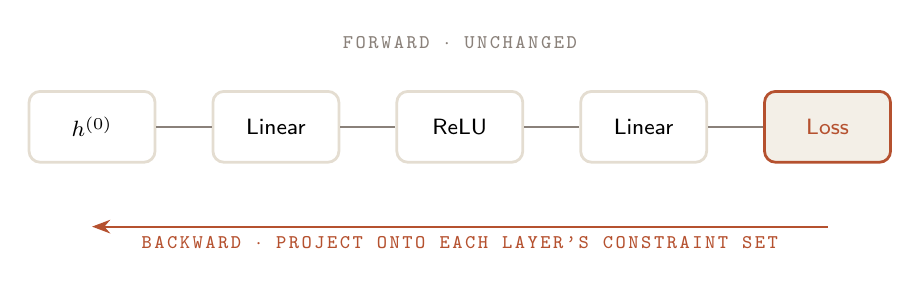
\begin{tikzpicture}[font=\footnotesize,>=Stealth,node distance=7mm]
    \tikzset{op/.style={draw=HAIR,rounded corners=4pt,fill=white,
              line width=1pt,minimum height=9mm,minimum width=16mm}}
    \node[op] (x) {$h^{(0)}$};
    \node[op,right=of x] (l1) {Linear};
    \node[op,right=of l1] (a) {ReLU};
    \node[op,right=of a] (l2) {Linear};
    \node[op,right=of l2,draw=TERRA,fill=PANEL,text=TERRA] (loss) {Loss};
    \draw[-,MUTE,thick] (x)--(l1); \draw[-,MUTE,thick] (l1)--(a);
    \draw[-,MUTE,thick] (a)--(l2); \draw[-,MUTE,thick] (l2)--(loss);
    \node[above=4mm of a] {\ttfamily\scriptsize\textls[120]{\color{MUTE}FORWARD $\cdot$ UNCHANGED}};
    \draw[->,TERRA,thick] ([yshift=-8mm]loss.south)--([yshift=-8mm]x.south)
      node[midway,below]{\ttfamily\scriptsize\textls[120]{\color{TERRA}BACKWARD $\cdot$ PROJECT ONTO EACH LAYER'S CONSTRAINT SET}};
  \end{tikzpicture}
  \end{center}
  \vfill
\end{frame}

% --- 10 · Residual is a gradient ---
\begin{frame}
  \vskip2pt
  \eyebrow{The idea}
  \slidetitle{The residual \itw{is} a gradient}
  \vskip10pt
  \begin{columns}[c,onlytextwidth]
    \begin{column}{0.56\textwidth}
      \[ \minimize_{\omega}\ F(\omega)=\sum_j f_j(\omega),\quad
         f_j=\tfrac12\,\dist^2(\tilde C_j,\cdot) \]
      \[ \nabla f_j(\omega)=\omega-\Pi_{\tilde C_j}(\omega) \]
      {\color{HAIR}\rule{\linewidth}{1pt}}
      \[ \bar\theta \leftarrow \theta-\alpha\bigl(\theta-\Pi_{\tilde C_j}(\theta)\bigr)
         =\theta-\alpha\,\nabla f_j(\theta) \]
      {\small\color{MUTE2}A plain projection step is an \textbf{incremental gradient step} --- wherever the projection is single-valued.}
    \end{column}
    \begin{column}{0.4\textwidth}
      \darkpanel{0.86\linewidth}{%
        \monolabel{TERRA2}{Nonlinear relaxation}\\[12pt]
        {\small\color{CREAMTXT}In \PT{} the residual populates \texttt{\textcolor{TERRA2}{.grad}}.}\\[12pt]
        {\small\color{CREAMMUT}Adam and Muon then treat the projection targets as \textcolor{CREAMTXT}{\textbf{adaptive, nonlinear relaxations}}.}}
    \end{column}
  \end{columns}
\end{frame}

% --- 11 · Demo / code ---
\begin{frame}[fragile]
  \vskip2pt
  \eyebrow{The idea}
  \slidetitle{A near drop-in replacement for PyTorch}
  \vskip8pt
  \begin{columns}[T,onlytextwidth]
    \begin{column}{0.49\textwidth}
      \tlabel{MUTE}{Standard PyTorch}\\[6pt]
      \begin{lstlisting}[style=pystd]
import torch.nn as nn
import torch.optim as optim

model = nn.Linear(784, 10)
criterion = nn.CrossEntropyLoss()
optimizer = optim.SGD(
    model.parameters(), lr=1.0)

logits = model(x)
criterion(logits, y).backward()
optimizer.step()
      \end{lstlisting}
    \end{column}
    \begin{column}{0.49\textwidth}
      \tlabel{TERRA}{PTorch}\\[6pt]
      \begin{lstlisting}[style=pyptorch]
import ptorch  (*@\textcolor{MUTE}{\# overrides torch}@*)
import ptorch.nn.modules as pnn
import ptorch.optim_static as poptim

model = pnn.Linear(784, 10)
criterion = pnn.CrossEntropy()
optimizer = poptim.ProjectionSGD(
    model.parameters(), lr=1.0)

logits = model(x)
criterion(logits, y).sum().backward() (*@\textcolor{TERRA2}{\# = projection!}@*)
optimizer.step()
      \end{lstlisting}
    \end{column}
  \end{columns}
  \vskip6pt
  {\small\color{MUTE2}Same training loop, swapped imports.\quad
   {\ttfamily\scriptsize\color{TERRA}python -m experiments.mlp.bench\_ptorch -{}-max-steps 50}}
\end{frame}

% ===================================================================
\section{Making it practical}
% ===================================================================
\divider{03}{Section 03}{Making it practical}{Killing the memory blow-up and bounding the backward signal.}

% --- 13 · Fused projections ---
\begin{frame}
  \vskip2pt
  \eyebrow{Making it practical}
  \slidetitle{Fused projections}
  \vskip10pt
  \begin{columns}[T,onlytextwidth]
    \begin{column}{0.47\textwidth}
      \tlabel{MUTE}{Problem}\\[6pt]
      {\small A linear-layer projection builds an
       $N_{\mathrm{in}}\!\times\! N_{\mathrm{out}}\!\times\! B$ tensor.}\\[10pt]
      {\color{TERRA}\rule{2pt}{3.4em}}\hspace{8pt}%
      \begin{minipage}[t]{0.84\linewidth}
        {\rmfamily\itshape\small\color{MUTE2}``The high memory demands of the 4-layer CNN
         necessitated reducing the hidden units to 16 to fit within 96\,GB GPU memory.''}\\[5pt]
        {\ttfamily\scriptsize\color{TERRA}--- PJAX}
      \end{minipage}
    \end{column}
    \begin{column}{0.47\textwidth}
      \tlabel{TERRA}{Idea}\\[6pt]
      {\small Projection composition is associative --- fuse the bilinear and consensus projections into one matmul.}
      \[ \bar\theta^{(i)}=\tfrac1B\bigl(\theta^{(i)}\odot(U\mathbf{1})+VH\bigr) \]
      \panel{0.92\linewidth}{\centering
        \tlabel{MUTE}{Peak memory}\\[6pt]
        $\mathcal{O}(N_{\mathrm{in}}N_{\mathrm{out}}B)\ \rightarrow\
         \mathcal{O}(N_{\mathrm{in}}B+N_{\mathrm{out}}B+N_{\mathrm{in}}N_{\mathrm{out}})$}
    \end{column}
  \end{columns}
  \vskip8pt
  {\small\color{MUTE2}Now trainable: a 32-64-128 CNN, a ResNet-8, and 2048-filter CNNs.
   Mix $\ell_2$ for big shared layers, $\ell_\infty$ elsewhere.}
\end{frame}

% --- 14 · Proximal projection ---
\begin{frame}
  \vskip2pt
  \eyebrow{Making it practical}
  \slidetitle{Proximal projection at the loss}
  \subt{The rigid snap $h^{(N)}\!\gets y$ is one extreme. Replace it by the proximal operator of the loss.}
  \vfill
  \begin{center}
    $\displaystyle h^{(N)}\gets\prox_{\lambda\mathcal{L}(\cdot,y)}\!\bigl(h^{(N)}\bigr)
      =\argmin_{u}\Bigl\{\mathcal{L}(u,y)+\tfrac{1}{2\lambda}\lVert u-h^{(N)}\rVert^2\Bigr\}$
  \end{center}
  \vfill
  \begin{columns}[T,onlytextwidth]
    \begin{column}{0.31\textwidth}
      {\color{TAN}\rule{\linewidth}{2.4pt}}\\[6pt]
      {\small Exactly one gradient step on the Moreau envelope $\mathcal{L}_\lambda$; the rigid snap is the $\lambda\!\to\!0$ limit.}
    \end{column}
    \begin{column}{0.31\textwidth}
      {\color{TAN}\rule{\linewidth}{2.4pt}}\\[6pt]
      {\small Same minimizers, but a \textbf{bounded} backward signal --- for MSE the residual contracts by $\tfrac{1}{1+\lambda}$.}
    \end{column}
    \begin{column}{0.31\textwidth}
      {\color{TERRA}\rule{\linewidth}{2.4pt}}\\[6pt]
      {\small Every constraint --- including the loss --- is now a single \textbf{differentiable} gradient step. With $K\!=\!1$, a true drop-in.}
    \end{column}
  \end{columns}
  \vfill
\end{frame}

% ===================================================================
\section{The limit \& the evidence}
% ===================================================================
\divider{04}{Section 04}{The limit, and the evidence}{A vanishing-target theorem --- and benchmarks from MLPs to a ViT.}

% --- 16 · Vanishing targets ---
\begin{frame}
  \vskip2pt
  \eyebrow{The limit \& the evidence}
  \slidetitle{Vanishing targets}
  \subt{Define the per-layer target magnitude\ \ $\delta^{(i)} := \lVert \bar h^{(i)}-h^{(i)}\rVert_2$.}
  \vskip8pt
  \begin{columns}[c,onlytextwidth]
    \begin{column}{0.52\textwidth}
      \darkpanel{0.9\linewidth}{%
        \monolabel{TERRA2}{Theorem $\cdot$ informal}\\[12pt]
        {\small\color{CREAMMUT}Under local non-expansiveness of the layer projection, for cyclic projections:}\\[12pt]
        \centering{\color{CREAMTXT}$\delta^{(0)}\le \delta^{(1)}\le \cdots \le \delta^{(N)}<\infty$}\\[12pt]
        \raggedright{\small\color{CREAMMUT}Strictly decreasing wherever a layer is actively learning.}}
    \end{column}
    \begin{column}{0.44\textwidth}
      \begin{itemize}\setlength{\itemsep}{0.7em}
        \item The signal to \textbf{early layers decays with depth}.
        \item A direct analogue of the \textbf{vanishing-gradient problem}.
      \end{itemize}
    \end{column}
  \end{columns}
\end{frame}

% --- 17 · Shallow MLP results ---
\begin{frame}
  \vskip2pt
  \eyebrow{The limit \& the evidence}
  \slidetitle{Shallow MLP: competitive with gradient descent}
  \subt{One hidden layer, 512 ReLU units. Baselines: Torch (gradient), PJAX (projection).}
  \vskip6pt
  \begin{columns}[c,onlytextwidth]
    \begin{column}{0.49\textwidth}\centering
      \figcard[width=0.9\linewidth,height=0.46\textheight,keepaspectratio]%
        {images/mlp/CIFAR10_1L_STEP.pdf}{CIFAR-10 --- accuracy vs.\ step}
    \end{column}
    \begin{column}{0.49\textwidth}\centering
      \figcard[width=0.9\linewidth,height=0.46\textheight,keepaspectratio]%
        {images/mlp/MNIST_1L_STEP.pdf}{MNIST --- accuracy vs.\ step}
    \end{column}
  \end{columns}
\end{frame}

% --- 18 · Depth degrades ---
\begin{frame}
  \vskip2pt
  \eyebrow{The limit \& the evidence}
  \slidetitle{Depth degrades projection-based training}
  \vskip8pt
  \begin{columns}[c,onlytextwidth]
    \begin{column}{0.55\textwidth}\centering
      \figcard[width=0.96\linewidth,height=0.5\textheight,keepaspectratio]%
        {images/deep/vanishing_combined.pdf}{$\delta$ decays away from the output; MSE worsens with depth}
    \end{column}
    \begin{column}{0.42\textwidth}
      \begin{itemize}\setlength{\itemsep}{0.6em}
        \item[\textcolor{TERRA}{\rule[0.16ex]{0.66ex}{0.66ex}}] \textbf{$\delta$ decays} away from the output; MSE worsens with depth.
        \item[\textcolor{TERRA}{\rule[0.16ex]{0.66ex}{0.66ex}}] Identity-recovery: layers $\ge 3$ from the output reach \textbf{machine precision} --- exactly as predicted.
        \item[\textcolor{TAN}{\rule[0.16ex]{0.66ex}{0.66ex}}] Muon-style orthogonalization stabilizes $\delta$ --- but no deep net yet beats a shallower one.
      \end{itemize}
    \end{column}
  \end{columns}
\end{frame}

% --- 19 · Beyond MLPs ---
\begin{frame}
  \vskip2pt
  \eyebrow{The limit \& the evidence}
  \slidetitle{Beyond MLPs: CNN and ViT}
  \vskip6pt
  \begin{columns}[T,onlytextwidth]
    \begin{column}{0.49\textwidth}\centering
      \figcard[width=0.88\linewidth,height=0.42\textheight,keepaspectratio]%
        {"images/other_benchmarks/CIFAR10_STEP (3).pdf"}{3-block CNN (32-64-128), CIFAR-10}\\[6pt]
      \raggedright{\small\color{MUTE2}\textbf{CNN.} Trainable via branch / add operators --- but underperforms its gradient counterpart. Depth again.}
    \end{column}
    \begin{column}{0.49\textwidth}\centering
      \figcard[width=0.88\linewidth,height=0.42\textheight,keepaspectratio]%
        {"images/other_benchmarks/attention_CIFAR10_STEP (2).pdf"}{Small ViT (4 blocks, 16 heads), CIFAR-10}\\[6pt]
      \raggedright{\small\color{MUTE2}\textbf{ViT.} $\approx$80\% train / 50\% val. Training a transformer at all is notable --- a proof of tractability, not yet efficiency.}
    \end{column}
  \end{columns}
\end{frame}

% ===================================================================
\section{Close}
% ===================================================================
\divider{05}{Section 05}{Close}{What was built --- and the two barriers that remain.}

% --- 21 · Contributions ---
\begin{frame}
  \vskip2pt
  \eyebrow{Close}
  \slidetitle{Contributions}
  \vfill
  \begin{minipage}{\linewidth}
    {\color{HAIR}\rule{\linewidth}{1pt}}\\[10pt]
    {\rmfamily\bfseries\fontsize{40}{40}\selectfont\color{TERRA}1}\hspace{18pt}%
    {\fontsize{17}{20}\selectfont A \textbf{PyTorch-native} projection framework.}\\[12pt]
    {\color{HAIR}\rule{\linewidth}{1pt}}\\[10pt]
    {\rmfamily\bfseries\fontsize{40}{40}\selectfont\color{TERRA}2}\hspace{18pt}%
    {\fontsize{17}{20}\selectfont Eliminating the memory overhead \& \textbf{closing the performance gap}.}\\[12pt]
    {\color{HAIR}\rule{\linewidth}{1pt}}\\[10pt]
    {\rmfamily\bfseries\fontsize{40}{40}\selectfont\color{TERRA}3}\hspace{18pt}%
    {\fontsize{17}{20}\selectfont A \textbf{vanishing-target theorem}.}\\[10pt]
    {\color{HAIR}\rule{\linewidth}{1pt}}
  \end{minipage}
  \vfill
\end{frame}

% --- 22 · Two barriers ---
\begin{frame}
  \vskip2pt
  \eyebrow{Close}
  \slidetitle{Two barriers, and an outlook}
  \vskip6pt
  {\rmfamily\itshape\fontsize{15}{19}\selectfont\color{MUTE2}Gradient-based learning won not because every early idea worked, but because enough were tried.}\par
  \vskip14pt
  \begin{columns}[T,onlytextwidth]
    \begin{column}{0.49\textwidth}
      \card[TERRA]{\linewidth}{%
        \tlabel{TERRA}{Barrier 01 $\cdot$ Depth}\\[8pt]
        {\small The target signal attenuates --- it needs projection analogues of \textbf{He initialization, batch norm, and skip connections}.}}
    \end{column}
    \begin{column}{0.49\textwidth}
      \card[TAN]{\linewidth}{%
        \tlabel{MUTE}{Barrier 02 $\cdot$ Coverage}\\[8pt]
        {\small Effective projections for \textbf{many architectures} are still unexplored.}}
    \end{column}
  \end{columns}
\end{frame}

% --- 23 · Thank you (full-bleed dark) ---
{\setbeamercolor{background canvas}{bg=INK}
\begin{frame}[plain]
  \begin{tikzpicture}[remember picture,overlay]
    \node[anchor=north east,inner sep=0pt]
      at ([xshift=40pt,yshift=24pt]current page.north east)
      {\rmfamily\fontsize{300}{300}\selectfont\color{WMDARK}$\bigcap$};
  \end{tikzpicture}%
  \vskip36pt
  \hspace{24pt}\rulebit{TERRA2}\hspace{8pt}\monolabel{TERRA2}{PTorch}\par
  \vfill
  \hspace{24pt}{\rmfamily\bfseries\fontsize{60}{62}\selectfont\color{CREAMTXT}Thank you}\par
  \vskip16pt
  \hspace{24pt}\begin{minipage}{0.78\textwidth}
    {\rmfamily\fontsize{20}{24}\selectfont\color{CREAMMUT}Narrowing the Gap Between Projection and Gradient-Based Learning}
  \end{minipage}\par
  \vskip26pt
  \hspace{24pt}{\color{WMDARK}\rule{0.9\textwidth}{1pt}}\par
  \vskip14pt
  \hspace{24pt}\begin{minipage}{0.9\textwidth}
    {\color{CREAMTXT}Jeff Cyuzuzo Jamb\'e}\hfill{\rmfamily\itshape\large\color{TERRA2}Questions?}
  \end{minipage}
  \vskip28pt
\end{frame}}

\end{document}
